% Classes of src/models/Glauber and their dependencies. Paper: section "Glauber model" (fig:glauber);
% Doxygen: GlauberGenerator.hpp.
%   pdflatex GlauberClasses.tex; pdftoppm -r 200 -png -singlefile GlauberClasses.pdf GlauberClasses;
%   pdftocairo -svg GlauberClasses.pdf GlauberClasses.svg
\documentclass[tikz,border=2pt]{standalone}
% Shared style of the class diagrams of CAP (figures/*Classes.tex): \input after \documentclass[tikz]{standalone}.
%  - boxes: blue = abstract base class, light blue = class, green = entry class of the folder (steering class, task),
%    yellow = free functions (tools), grey = class of another folder;
%  - arrows: open triangle = inherits from; dashed with diamond = owns (holds); dashed with arrow = uses.
\usepackage[scaled=0.92]{helvet}
\usetikzlibrary{arrows.meta,shapes.multipart,positioning,fit,backgrounds,calc}
\renewcommand{\familydefault}{\sfdefault}
\definecolor{abstract}{HTML}{D6E4F5}
\definecolor{concrete}{HTML}{EEF4FB}
\definecolor{steer}{HTML}{DCEFD9}
\definecolor{tools}{HTML}{FFF8E6}
\definecolor{external}{HTML}{E9E9E9}
\definecolor{dependline}{HTML}{8A6D3B}
\definecolor{folder}{HTML}{F7F7F7}
\tikzset{
  every picture/.style={font=\scriptsize},
  cls/.style={draw, fill=concrete, align=center, inner sep=2.5pt, text width=#1, font=\tiny},
  cls/.default=3.0cm,
  abs/.style={cls=#1, fill=abstract},
  abs/.default=3.0cm,
  steer/.style={cls=#1, fill=steer, line width=0.8pt},
  steer/.default=4.2cm,
  tool/.style={cls=#1, fill=tools},
  tool/.default=4.2cm,
  ext/.style={cls=#1, fill=external, dashed},
  ext/.default=2.6cm,
  fam/.style={draw, rectangle split, rectangle split parts=2, rectangle split part fill={#1,white},
              rectangle split part align={center,left}, inner sep=2.5pt, align=left},
  inherit/.style={-{Triangle[open,length=2.2mm,width=2.2mm]}, thin},
  uses/.style={dashed, dependline, -{Stealth[length=1.6mm]}, thin},
  owns/.style={dashed, dependline, {Diamond[length=2.4mm,width=1.6mm]}-, thin},
  lbl/.style={font=\tiny, text=dependline, align=center},
  note/.style={font=\tiny, align=left, text=black!70},
  title/.style={font=\footnotesize\bfseries, anchor=north west},
}
% a member line in a class box
\newcommand{\m}[1]{\\#1}
\newcommand{\cn}[1]{{\scriptsize\textbf{#1}}}
\newcommand{\an}[1]{{\scriptsize\textbf{\textit{#1}}}}

% legend common to the class diagrams (place with \legendat{x}{y})
\newcommand{\legendat}[2]{%
  \begin{scope}[shift={(#1,#2)}, font=\tiny]
    \node[abs=0.9cm, minimum height=3mm, inner sep=1pt] (lA) at (0,0) {abstract};
    \node[cls=0.9cm, minimum height=3mm, inner sep=1pt, right=1mm of lA] (lC) {class};
    \node[steer=1.1cm, minimum height=3mm, inner sep=1pt, right=1mm of lC] (lS) {entry class};
    \node[tool=1.1cm, minimum height=3mm, inner sep=1pt, right=1mm of lS] (lT) {functions};
    \node[ext=1.3cm, minimum height=3mm, inner sep=1pt, right=1mm of lT] (lE) {other folder};
    \draw[inherit] ($(lE.east)+(1mm,0)$) -- ++(5mm,0) node[right, inner sep=1pt] (l1) {inherits};
    \draw[owns] ($(l1.east)+(1mm,0)$) -- ++(5mm,0) node[right, inner sep=1pt] (l2) {owns};
    \draw[uses] ($(l2.east)+(1mm,0)$) -- ++(5mm,0) node[right, inner sep=1pt] {uses};
  \end{scope}}

\begin{document}
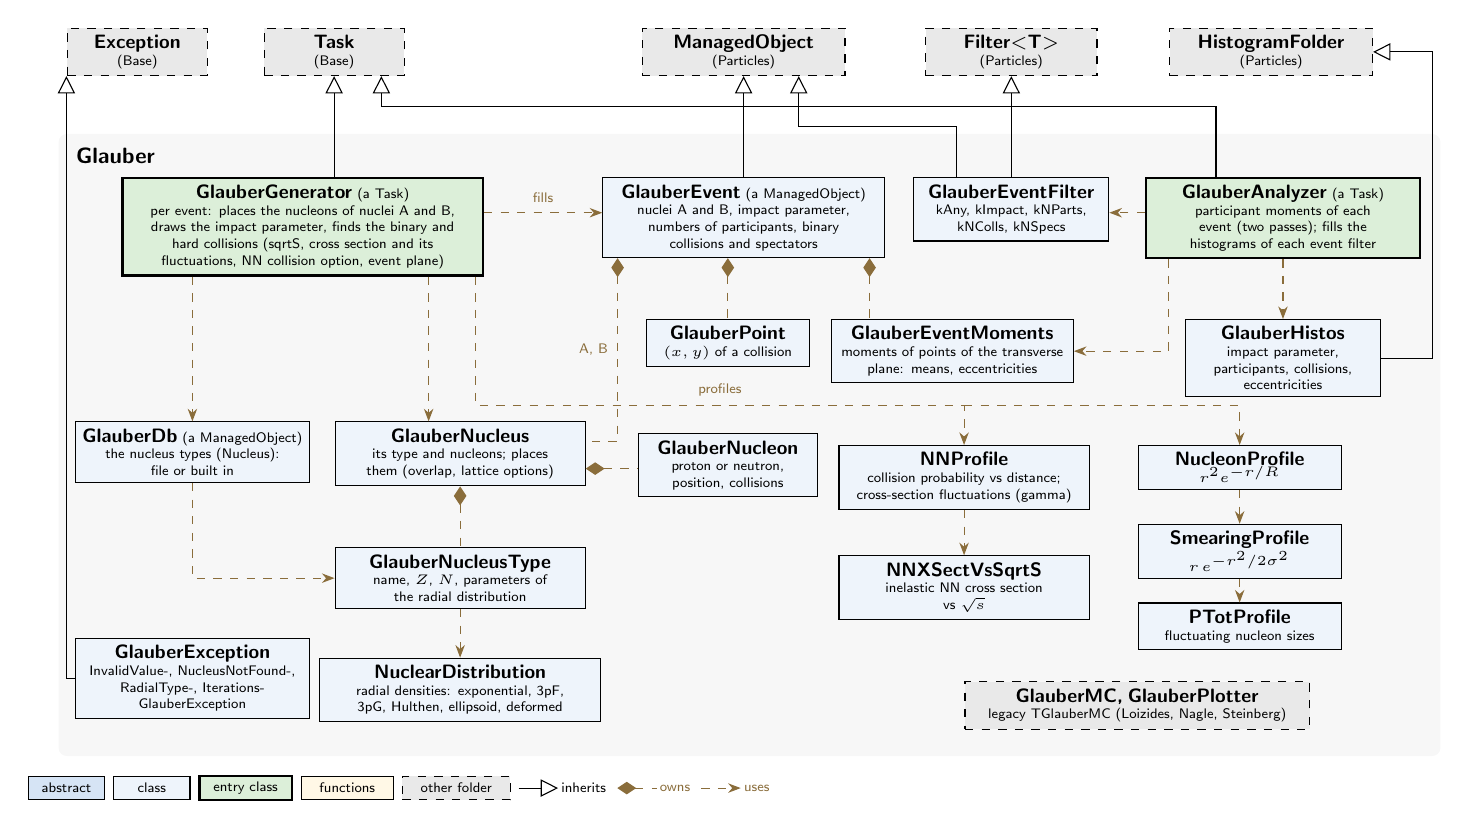
\begin{tikzpicture}[every node/.append style={anchor=north}]
  \begin{scope}[on background layer]
    \fill[folder, rounded corners=3pt] (-0.1,-1.05) rectangle (17.45,-8.95);
  \end{scope}
  \node[title] at (0.0,-1.1) {Glauber};

  % other folders
  \node[ext=1.6cm] (Exc) at (0.9,0.3) {\cn{Exception}\m{(Base)}};
  \node[ext=1.6cm] (Task) at (3.4,0.3) {\an{Task}\m{(Base)}};
  \node[ext=2.4cm] (MO) at (8.6,0.3) {\an{ManagedObject}\m{(Particles)}};
  \node[ext=2.0cm] (Filter) at (12.0,0.3) {\an{Filter$<$T$>$}\m{(Particles)}};
  \node[ext=2.4cm] (HF) at (15.3,0.3) {\an{HistogramFolder}\m{(Particles)}};

  % tasks and events
  \node[steer=4.4cm] (Gen) at (3.0,-1.6)
    {\cn{GlauberGenerator} \tiny(a Task)\m{per event: places the nucleons of nuclei A and B,}
     \m{draws the impact parameter, finds the binary and}\m{hard collisions (sqrtS, cross section and its}
     \m{fluctuations, NN collision option, event plane)}};
  \node[cls=3.4cm] (Event) at (8.6,-1.6)
    {\cn{GlauberEvent} \tiny(a ManagedObject)\m{nuclei A and B, impact parameter,}\m{numbers of participants, binary}\m{collisions and spectators}};
  \node[cls=2.3cm] (EF) at (12.0,-1.6) {\cn{GlauberEventFilter}\m{kAny, kImpact, kNParts,}\m{kNColls, kNSpecs}};
  \node[steer=3.3cm] (Ana) at (15.45,-1.6)
    {\cn{GlauberAnalyzer} \tiny(a Task)\m{participant moments of each}\m{event (two passes); fills the}\m{histograms of each event filter}};
  \draw[inherit] (Gen.north -| Task.south) -- (Task.south);
  \draw[inherit] (14.6,0 |- Ana.north) |- (4.0,-0.7) -- (4.0,0 |- Task.south);
  \draw[inherit] (Event.north) -- (MO.south);
  \draw[inherit] (EF.north) -- (Filter.south);
  \draw[inherit] (11.3,0 |- EF.north) |- (9.3,-0.95) -- (9.3,0 |- MO.south);
  \draw[uses] (Gen.east |- 0,-2.05) -- node[lbl, above]{fills} (Event.west |- 0,-2.05);
  \draw[uses] (Ana.west |- 0,-2.05) -- (EF.east |- 0,-2.05);

  \node[cls=1.9cm] (Point) at (8.4,-3.4) {\cn{GlauberPoint}\m{$(x, y)$ of a collision}};
  \node[cls=2.9cm] (Mom) at (11.25,-3.4) {\cn{GlauberEventMoments}\m{moments of points of the transverse}\m{plane: means, eccentricities}};
  \node[cls=2.3cm] (Histos) at (15.45,-3.4) {\cn{GlauberHistos}\m{impact parameter,}\m{participants, collisions,}\m{eccentricities}};
  \draw[owns] (8.4,0 |- Event.south) -- (Point.north);
  \draw[owns] (10.2,0 |- Event.south) -- (10.2,0 |- Mom.north);
  \draw[uses] (Ana.south) -- (Histos.north);
  \draw[uses] (14.0,0 |- Ana.south) |- (Mom.east);
  \draw[inherit] (Histos.east) -- (17.35,0 |- Histos.east) |- (HF.east);

  % nuclei
  \node[cls=2.8cm] (Db) at (1.6,-4.7) {\cn{GlauberDb} \tiny(a ManagedObject)\m{the nucleus types (Nucleus):}\m{file or built in}};
  \node[cls=3.0cm] (Nucleus) at (5.0,-4.7)
    {\cn{GlauberNucleus}\m{its type and nucleons; places}\m{them (overlap, lattice options)}};
  \node[cls=2.1cm] (Nucleon) at (8.4,-4.85) {\cn{GlauberNucleon}\m{proton or neutron,}\m{position, collisions}};
  \node[cls=3.0cm] (NType) at (5.0,-6.3) {\cn{GlauberNucleusType}\m{name, $Z$, $N$, parameters of}\m{the radial distribution}};
  \node[cls=3.4cm] (ND) at (5.0,-7.7) {\cn{NuclearDistribution}\m{radial densities: exponential, 3pF,}\m{3pG, Hulthen, ellipsoid, deformed}};
  \draw[uses] (1.6,0 |- Gen.south) -- (Db.north);
  \draw[uses] (4.6,0 |- Gen.south) -- (4.6,0 |- Nucleus.north);
  \draw[owns] (7.0,0 |- Event.south) |- node[lbl, pos=0.25, left]{A, B} (Nucleus.east |- 0,-4.95);
  \draw[owns] (Nucleus.east |- 0,-5.3) -- (Nucleon.west |- 0,-5.3);
  \draw[owns] (Nucleus.south) -- (NType.north);
  \draw[uses] (NType.south) -- (ND.north);
  \draw[uses] (Db.south) |- (NType.west);

  % profiles
  \node[cls=3.0cm] (NN) at (11.4,-5.0) {\cn{NNProfile}\m{collision probability vs distance;}\m{cross-section fluctuations (gamma)}};
  \node[cls=3.0cm] (XS) at (11.4,-6.4) {\cn{NNXSectVsSqrtS}\m{inelastic NN cross section}\m{vs $\sqrt{s}$}};
  \node[cls=2.4cm] (NP) at (14.9,-5.0) {\cn{NucleonProfile}\m{$r^2 e^{-r/R}$}};
  \node[cls=2.4cm] (SP) at (14.9,-6.0) {\cn{SmearingProfile}\m{$r\, e^{-r^2/2\sigma^2}$}};
  \node[cls=2.4cm] (PT) at (14.9,-7.0) {\cn{PTotProfile}\m{fluctuating nucleon sizes}};
  \draw[uses] (5.2,0 |- Gen.south) |- node[lbl, pos=0.75, above]{profiles} (11.4,-4.5) -- (NN.north);
  \draw[uses] (11.4,-4.5) -| (NP.north);
  \draw[uses] (NN.south) -- (XS.north);
  \draw[uses] (NP.south) -- (SP.north);
  \draw[uses] (SP.south) -- (PT.north);

  % exceptions and legacy
  \node[cls=2.8cm] (GExc) at (1.6,-7.45) {\cn{GlauberException}\m{InvalidValue-, NucleusNotFound-,}\m{RadialType-, Iterations-}\m{GlauberException}};
  \draw[inherit] (GExc.west) -- (0.0,0 |- GExc.west) -- (0.0,0 |- Exc.south) ;
  \node[ext=4.2cm] (Legacy) at (13.6,-8.0) {\cn{GlauberMC, GlauberPlotter}\m{legacy TGlauberMC (Loizides, Nagle, Steinberg)}};
  \legendat{0.0}{-9.2}
\end{tikzpicture}
\end{document}
